% $Id: introduction.tex 87303 2016-02-08 13:44:29Z lafferty $

\subsection{Reconstruction and selection}
\label{subsec:selection}

Pairs of muon candidates are reconstructed combining opposite-charged tracks with hits in the vertex locator (VELO), trigger tracker, tracker stations, and muon chambers. 
In addition, the tracks are required to be separated by at least $6\sigma$ from any $p-p$ collision point in the event.
Tracks with transverse momentum lower than 80\mevc are ignored. 
A dimuon candidate pair can be combined with a $\pi^0$ candidate to build a \KS\ candidate. 
The events in which the entire decay chain is used are classified as FULL. When only the dimuon information is used, they are clasified as PARTIAL.

Neutral pion candidates are reconstructed from 
$\gamma$ candidate pairs that correspond to two independent clusters in the calorimeter.
Each photon candidate is required to have a transverse momentum of
at least 200\mevc and the pion candidate a mass within 30\mevcc of the world average $\pi^0$ mass.
The mass resolution is then improved by constraining the $\pi^0$ candidate 
mass to the world average $\pi^0$ mass, and by constraining the three-momentum
vector of the \KS to point back to the production vertex. For the PARTIAL candidates, a momentum vector with an absolute value of $\approx 10\gevc$
is used as a representative of the $\pi^0$ momentum when calculating the invariant mass. As a consequence of these kinematic constraints, the \KS\ candidate 
mass resolution depends only weakly on the $\pi^{0}$ momentum.

Additional selection requirements are applied to reduce the
amount of data to analyze, fulfil the rate requirements for LHCb offline
processing and reduce the amount of background. These include a \KS\ candidate lifetime of at least $1\;\rm ps$
and removing events in the kinematic region of $\Lambda\to p \pi$ and $\KS\to \pi^{+}\pi^{-}$ in the Armenteros-Podolanski plane~\cite{Armenteros}.
The total reconstruction and selection efficiency for the FULL channel is $5.47\times10^{-4}$.

Requiring a well-reconstructed  $\pi^0$ implies an inefficiency penalty of a factor ten.
Thus, a complementary strategy for the PARTIAL candidates is also investigated.
Indeed, the constraints on the $\pi^0$ mass and the \KS momentum are sufficient to create a peaking distribution if there is an estimate of the typical
value of the $\pi^0$ momentum ($\approx 10\gevc$), as shown in \figref{fig:peaks}.
A comparison of the reconstructed mass resolution between FULL and PARTIAL is difficult due to the asymmetric and non-Gaussian distribution of the PARTIAL case. To get an estimate, the corresponding 
FWHM values are calculated. In the FULL case, it is 23.3~\mevcc and in the PARTIAL 40.6~\mevcc.

The PARTIAL selection does not require any information about a reconstructed $\pi^0$. Some
requirements had to be tightened in order to keep the background at a manageable level. These include a lower distance of closest approach between the two
muon tracks; a minimum requirement on the \KS\ vertex quality, $\chi^{2}/ndof = 9$; a higher minimum requirement on the \KS\ vertex detachment from the interaction point;
and minimum radial, $z$- and absolute distance requirements between the \KS\ vertex and the interaction point.
The total reconstruction and selection efficiency for the PARTIAL analysis is $3.0\times 10^{-3}$ , well above that of the FULL,
but at a cost of an increased background yield.

\begin{figure} [htb!]
\begin{center}
%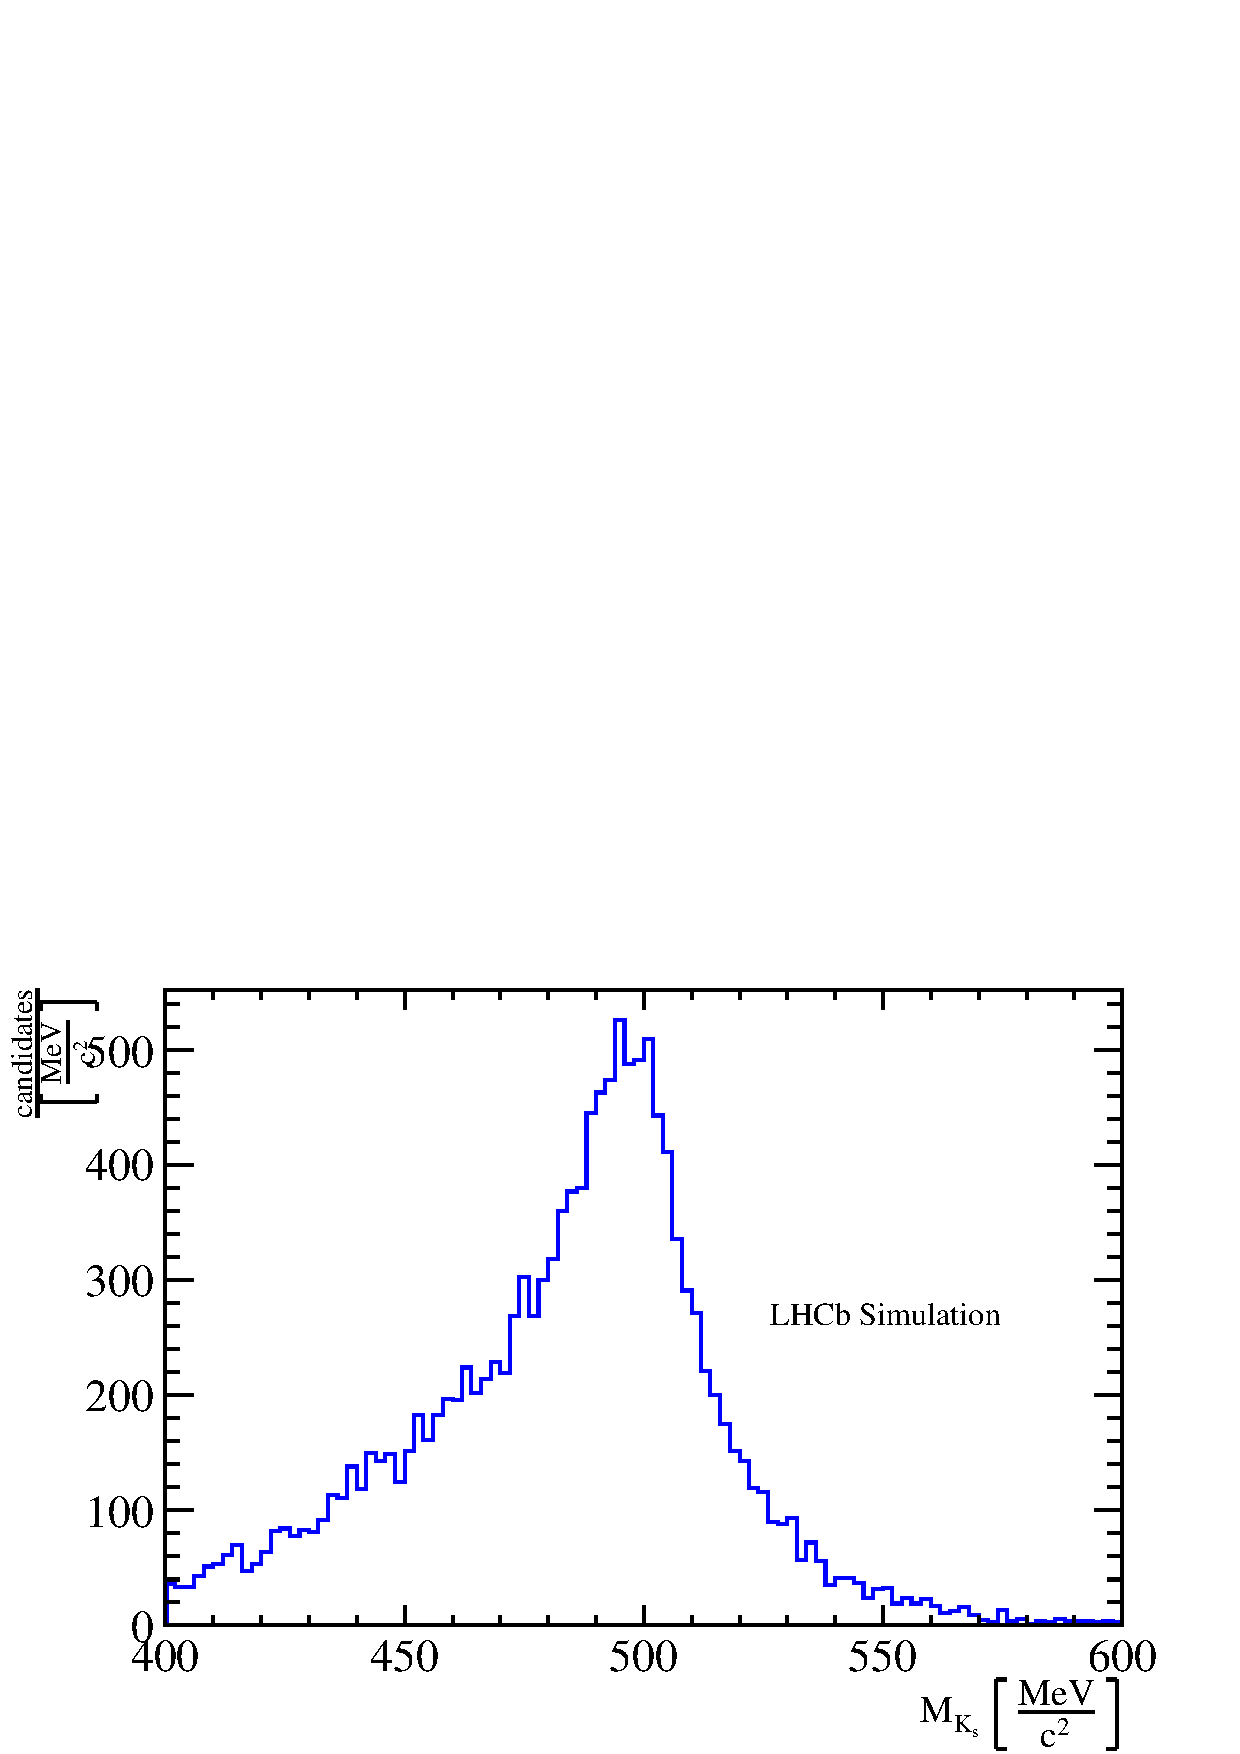
\includegraphics[scale=0.35]{figs/hphantom.pdf}
\includegraphics[scale=0.6]{figs/Kspi0MuMu/M_V0_vs_VC.pdf}
\caption{Comparison between the FULL (solid red) and PARTIAL (dashed green) kaon candidate mass distributions. \label{fig:peaks}}
\end{center}
\end{figure}

A BDT is used to separate signal from combinatorial background. It is trained with MC events (signal class) and a part of the data that is not used in the fit
(combinatorial background class). The BDT uses information about the geometrical properties of the events,
kinematics, track quality, and muon identification quality. The BDT response for signal and background for both FULL and PARTIAL 
is shown in \figref{fig:BDT}.


\begin{figure} [htb!]
\begin{center}
\includegraphics[scale=0.38]{figs/Kspi0MuMu/BDT_sig_vs_bkg_FULL.pdf}%BDTFULL.pdf}
\includegraphics[scale=0.38]{figs/Kspi0MuMu/BDT_sig_vs_bkg_PARTIAL.pdf}%BDTPARTIAL.pdf}
\caption{BDT response both for signal (solid red) and background (dashed black). Right: FULL channel. Left: PARTIAL channel.  Signal and background are normalized to the same area. \label{fig:BDT}}
\end{center}
\end{figure}


The events are classified in four bins of the BDT response. The signal yields are obtained in a simultaneous fit 
of the mass distribution in each BDT bin, as described in the following sections.
